%!TEX root=../document.tex

\section{Ergebnisse}
\label{sec:Ergebnisse}
\subsection{Designüberlegungen}
Grundsätzlich wurden beim Server und Client die Aufgaben in Kryptographie und Übertragung geteilt. Somit gibt es insgesamt 4 Klassen, wobei die Netzwerkobjekte schlussendlich die \texttt{main}-Funktion enthalten und auf die Verschlüsselungsfunktionalitäten der \texttt{SecureXXX} Klassen zurückgreifen.
Das Klassendiagramm sieht schlussendlich wie folgt aus:\

\begin{figure}[!h]
	\begin{center}
		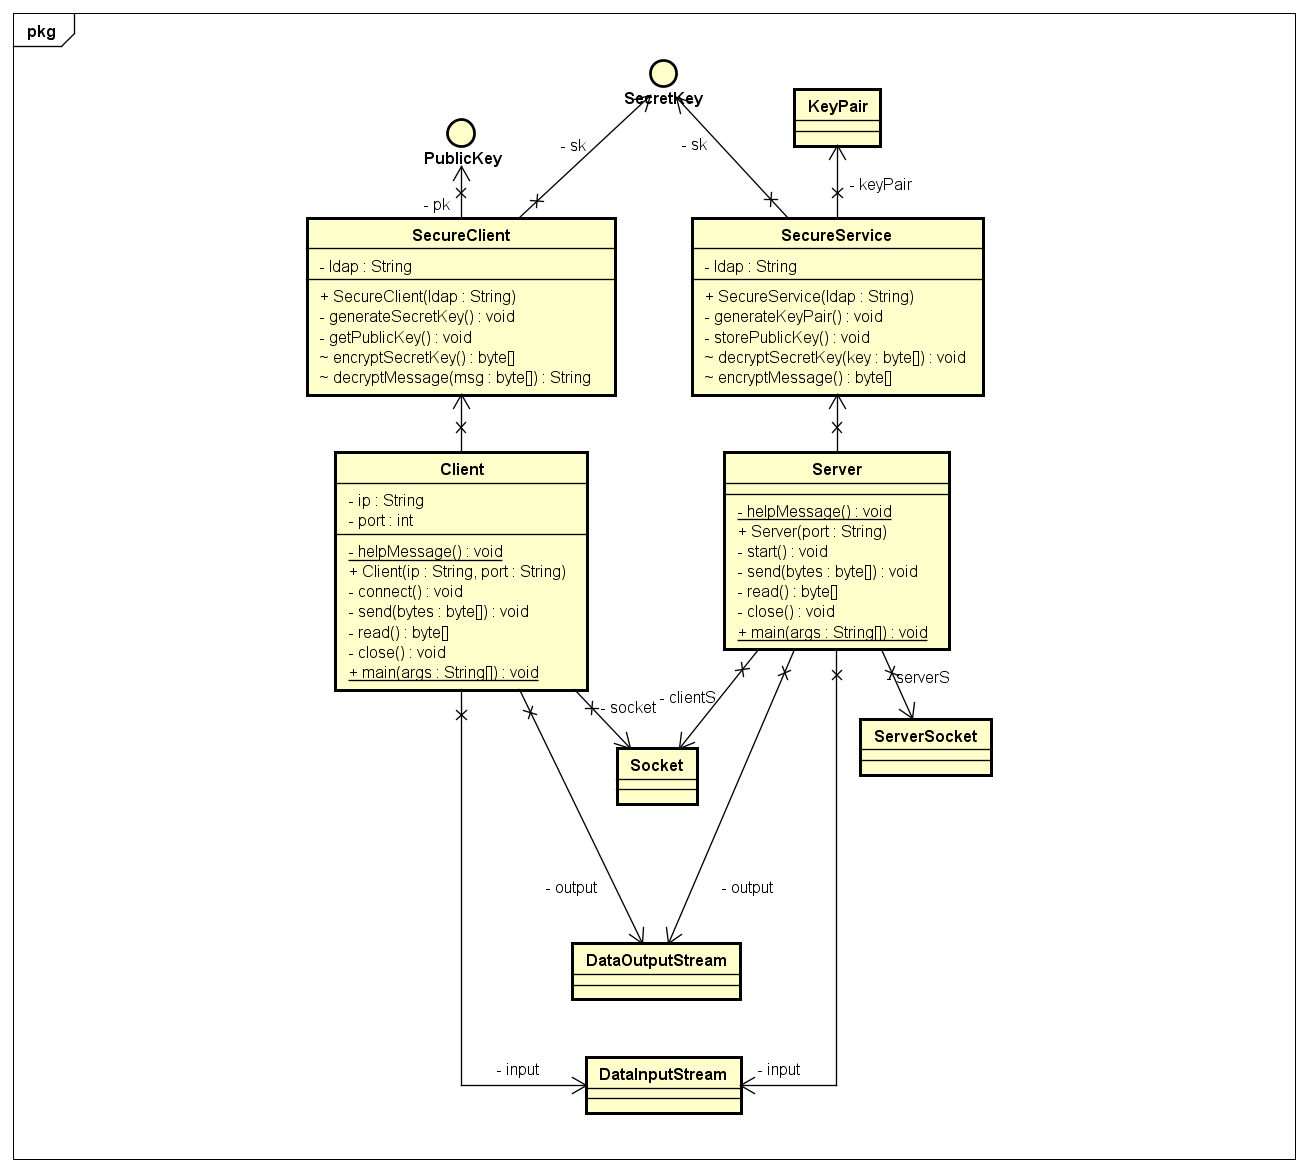
\includegraphics[width=0.9\linewidth]{images/class_diagram.png}
		\caption{UML - Klassendiagramm}
		\label{classd}
	\end{center}
\end{figure}
Die Methoden in den \texttt{SecureXXX} Klassen wurden unter der Vorgabe des Ablaufdiagramms (Abbildung~\ref{ablauf}) auf Seite~\pageref{ablauf} entworfen.
\clearpage
Der Ablauf der Methoden ist selbsterklärend:
\begin{itemize}
	\item \texttt{\underline{SecureService:} generateKeyPair()}
	\item \texttt{\underline{SecureService:} storePublicKey()}
	\item \texttt{\underline{SecureClient:} generateSecretKey()}
	\item \texttt{\underline{SecureClient:} getPublicKey()}
	\item \texttt{\underline{SecureClient:} encryptSecretKey()}
	\item \texttt{\underline{SecureService:} decryptSecretKey()}
	\item \texttt{\underline{SecureService:} encryptMessage()}
	\item \texttt{\underline{SecureClient:} decryptMessage()}
\end{itemize}
Die Kommunikationsklassen sorgen nur noch für das Senden und Empfangen, sowie das Verwalten des \texttt{ServerSockets} und \texttt{Sockets}.
\subsection{Kommunikation}
Als Kommunikationsart wurde IPC gewählt, da diese einfach zu realisieren ist.

Da die kryptographischen Java-Libraries direkt mit \texttt{byte}-Arrays arbeiten, wurde auf \texttt{PrintWriter} und sonstige Klassen, die bei der IPC Laborübung des Vorjahres verwendet wurden, verzichtet.

Die Datenübertragung funktioniert wie folgt:
\begin{lstlisting}[style=Java, caption=Senden per \texttt{DataOutputStream}]
private void send(byte[] bytes) {
	try {
		output.writeInt(bytes.length);
		output.write(bytes);
	} catch (IOException e) {
		System.err.println("Couldn't send data: " + e.getMessage());
		System.exit(1);
	}
}
\end{lstlisting}
Hierbei wird zuerst die Länge der zu schreibenden Daten festgelegt und danach werden die Daten geschrieben.

Analog dazu funktioniert das Empfangen von Daten:
\begin{lstlisting}[style=Java, caption=Empfangen per \texttt{DataInputStream}]
private byte[] read() {
	try {
		byte[] message = new byte[input.readInt()];
		input.readFully(message, 0, message.length);
		return message;
	} catch (IOException e) {
		System.err.println("Couldn't receive data: " + e.getMessage());
		System.exit(1);
		return null;
	}
}
\end{lstlisting}
Auf das Speichern und Lesen bezüglich LDAP Verzeichnisdienste wird nicht näher eingegangen, da dies nicht Thema der Übung ist und bereits im letzten Jahr behandelt wurde.

Wichtig für diese Übung war nur, dass man sich für das Manipulieren eines Attributs authentifizieren muss, für das Auslesen jedoch nicht.
\subsection{Schlüsselpaar erstellen}
Der erste Schritt des hybriden Verschlüsselungsverfahren ist, ein Schlüsselpaar zu generieren.
\begin{lstlisting}[style=Java, caption=Generieren eines Schlüsselpaars]
// setting up key pair generator
KeyPairGenerator generator = KeyPairGenerator.getInstance("RSA");
// generating randomness securely
SecureRandom random = SecureRandom.getInstance("SHA1PRNG", "SUN");
// initialize generator with 2048 bit key size
generator.initialize(2048, random);
// generating key pair
keyPair = generator.generateKeyPair();
\end{lstlisting}
Dazu wird zuerst ein \texttt{KeyPairGenerator} mit dem gewünschten Algorithmus erstellt. Mögliche Werte wären hier auch EC (elliptische Kurven), DSA (für Signaturen) oder Diffie-Hellman.

Danach wird ein ``Zufallsgenerator'' erstellt, der so konfiguriert ist, dass er eine plattformunabhängige Implementierung verwendet. Andere mögliche Algorithmen greifen auf Funktionalitäten des OS zurück.

Anschließend wird der Schlüsselgenerator mit einer Key-Größe von 2048-bit und dem ``Zufallsgenerator'' initialisiert.

Zuletzt wird das eigentliche Schlüsselpaar erzeugt.
\subsection{Übertragung des \texttt{PublicKey}}
Der Schlüssel wird in dem LDAP Verzeichnisdienst als hexadezimaler Wert gespeichert.
\begin{lstlisting}[style=Java, caption=Hexadezimale String-Darstellung des \texttt{PublicKey}]
DatatypeConverter.printHexBinary(keyPair.getPublic().getEncoded());
\end{lstlisting}
Der Client muss diesen String auslesen und zu einem \texttt{PublicKey} Objekt umwandeln.
\clearpage
\begin{lstlisting}[style=Java, caption=Umwandlung eines Strings zu einem gültigen \texttt{PublicKey}]
// get binary array from hex string
byte[] key = DatatypeConverter.parseHexBinary(response);
// key specifications
X509EncodedKeySpec pubKeySpec = new X509EncodedKeySpec(key);
// key factory for RSA
KeyFactory keyFactory = KeyFactory.getInstance("RSA");
// generate public key from the specification
pk = keyFactory.generatePublic(pubKeySpec);
\end{lstlisting}
Zuerst wird der String wieder in ein \texttt{byte}-Array umgewandelt.

Danach wird die ``Codierungsspezifikation'' erstellt, welche die Codierungsinformationen nach dem X.509 Standard enthält.

Nun wird eine \texttt{KeyFactory} für den RSA Algorithmus erstellt.

Zuletzt decodiert die \texttt{KeyFactory} mit Hilfe der Codierungsspezifikationen den \texttt{PublicKey}.
\subsection{\texttt{SecretKey} erstellen}
Das Erstellen des \texttt{SecretKey} ist simpel.
\begin{lstlisting}[style=Java, caption=Erstellen des \texttt{SecretKey}]
// setting the algorithm
KeyGenerator keygen = KeyGenerator.getInstance("AES");
// actual generating
sk = keygen.generateKey();
\end{lstlisting}
Zuerst wird wieder der Algorithmus gewählt und danach wird der Schlüssel generiert. Mögliche Werte wären zum Beispiel Blowfish, DES oder HmacSHA512.
\subsection{\texttt{SecretKey} mit dem \texttt{PublicKey} verschlüsseln}
\begin{lstlisting}[style=Java, caption=\texttt{SecretKey} mit dem \texttt{PublicKey} verschlüsseln]
// setting up the cipher
Cipher cipher = Cipher.getInstance("RSA");
cipher.init(Cipher.ENCRYPT_MODE, pk);
// encrypt the secret key
return cipher.doFinal(sk.getEncoded());
\end{lstlisting}
Der Cipher transformiert (verschlüsselt) Information mit Hilfe eines bestimmten Algorithmus (hier RSA) und eines Keys (\texttt{PublicKey}). Dazu wird der Cipher in den Verschlüsselungsmodus gesetzt und schon kann verschlüsselt werden.
\clearpage
\subsection{\texttt{SecretKey} mit dem \texttt{PrivateKey} entschlüsseln}
\begin{lstlisting}[style=Java, caption=\texttt{SecretKey} mit dem \texttt{PrivateKey} entschlüsseln]
// setting up cipher for decryption
Cipher cipher = Cipher.getInstance("RSA");
cipher.init(Cipher.DECRYPT_MODE, keyPair.getPrivate());
// decrypting
byte[] ready = cipher.doFinal(key);
sk = new SecretKeySpec(ready, 0, ready.length, "AES");
\end{lstlisting}
Diese Methode funktioniert analog zur vorherigen. Zusätzlich muss beim Konvertieren des \texttt{byte}-Arrays angegeben werden, um welche Schlüsselart (AES) es sich handelt.
\subsection{Nachricht mit dem \texttt{SecretKey} verschlüsseln}
\begin{lstlisting}[style=Java, caption=symmetrische Verschlüsselung]
// setting up cipher for encryption
Cipher cipher = Cipher.getInstance("AES");
cipher.init(Cipher.ENCRYPT_MODE, sk);
// encrypt
return cipher.doFinal(message.getBytes());
\end{lstlisting}
Wie man sieht, gibt es keinen programmiertechnischen Unterschied beim Verwenden eines Ciphers mit asymmetrischer oder symmetrischer Verschlüsselung.
\subsection{Nachricht mit dem \texttt{SecretKey} entschlüsseln}
\begin{lstlisting}[style=Java, caption=symmetrische Entschlüsselung]
// setting up the decrypting cipher
Cipher cipher = Cipher.getInstance("AES");
cipher.init(Cipher.DECRYPT_MODE, sk);
// decrypting
byte[] ready = cipher.doFinal(msg);
return new String(ready);
\end{lstlisting}
Zusätzlich wird die Nachricht am Schluss wieder in einen String verwandelt.
\subsection{Testfälle}
mit usage
\subsection{Tabelle}
\renewcommand{\arraystretch}{1.5}
\begin{table}[!h]
	\center
	\begin{tabular}{ | @{\hspace{3mm}} c @{\hspace{3mm}} | @{\hspace{3mm}} l @{\hspace{3mm}} | }
		\hline Header & Kopf\\ \hline\hline
		\textbf{Lorem} & Ipsum dolor sit amet, consetetur sadipscing elitr\\ \hline
		\textbf{Ipsum} & At vero eos et accusam et justo duo dolores et ea rebum.\\
			& Stet clita kasd gubergren, no sea takimata sanctus\\ \hline
		\textbf{Dolor} & Consetetur sadipscing elitr, sed diam nonumy\\\hline
	\end{tabular}
	\caption{Lorem ipsum dolor sit amet \cite{tanenbaum2007verteilte}}
	\label{methoden}
\end{table}

\subsection{Aufzählung}

\begin{itemize}
	\item \textbf{Lorem ipsum:} dolor sit amet, consetetur sadipscing elitr
	\item sed diam nonumy eirmod tempor invidunt ut labore et dolore magna aliquyam erat
	\item ut labore et dolore magna aliquyam erat, sed diam voluptua
\end{itemize}

\subsection{Code}

At vero eos et accusam et justo duo dolores et ea rebum.

\begin{lstlisting}[style=Java, caption=Implizite Transaktion \cite{tanenbaum2007verteilte}]
try{
   gTransCur.begin();
   //Perform the operation inside the transaction
   not_registered = 
       gRegistrarObjRef.register_for_courses(student_id,selected_course_numbers);


   if (not_registered != null)

     //If operation executes with no errors, commit the transaction
     boolean report_heuristics = true;
     gTransCur.commit(report_heuristics);

   } else gTransCur.rollback();


} catch(org.omg.CosTransactions.NoTransaction nte) {
    System.err.println("NoTransaction: " + nte);
    System.exit(1);
} catch(org.omg.CosTransactions.SubtransactionsUnavailable e) {
    System.err.println("Subtransactions Unavailable: " + e);
    System.exit(1);
} catch(org.omg.CosTransactions.HeuristicHazard e) {
    System.err.println("HeuristicHazard: " + e);
    System.exit(1);
} catch(org.omg.CosTransactions.HeuristicMixed e) {
    System.err.println("HeuristicMixed: " + e);
    System.exit(1);
}
\end{lstlisting}

